% --------------------------------------------------------------------------- %
% Poster for the ECCS 2011 Conference about Elementary Dynamic Networks.      %
% --------------------------------------------------------------------------- %
% Created with Brian Amberg's LaTeX Poster Template. Please refer for the     %
% attached README.md file for the details how to compile with `pdflatex`.     %
% --------------------------------------------------------------------------- %
% $LastChangedDate:: 2011-09-11 10:57:12 +0200 (V, 11 szept. 2011)          $ %
% $LastChangedRevision:: 128                                                $ %
% $LastChangedBy:: rlegendi                                                 $ %
% $Id:: poster.tex 128 2011-09-11 08:57:12Z rlegendi                        $ %
% --------------------------------------------------------------------------- %
\documentclass[a0paper,portrait]{baposter}

\usepackage{relsize}		% For \smaller
\usepackage{url}			% For \url
\usepackage{epstopdf}	% Included EPS files automatically converted to PDF to include with pdflatex
\usepackage{enumitem}

%%% Global Settings %%%%%%%%%%%%%%%%%%%%%%%%%%%%%%%%%%%%%%%%%%%%%%%%%%%%%%%%%%%

\graphicspath{{pix/}}	% Root directory of the pictures 
\tracingstats=2			% Enabled LaTeX logging with conditionals

%%% Color Definitions %%%%%%%%%%%%%%%%%%%%%%%%%%%%%%%%%%%%%%%%%%%%%%%%%%%%%%%%%

\definecolor{bordercol}{RGB}{40,40,40}
\definecolor{headercol1}{RGB}{186,215,230}
\definecolor{headercol2}{RGB}{80,80,80}
\definecolor{headerfontcol}{RGB}{0,0,0}
\definecolor{boxcolor}{RGB}{186,215,230}

%%%%%%%%%%%%%%%%%%%%%%%%%%%%%%%%%%%%%%%%%%%%%%%%%%%%%%%%%%%%%%%%%%%%%%%%%%%%%%%%
%%% Utility functions %%%%%%%%%%%%%%%%%%%%%%%%%%%%%%%%%%%%%%%%%%%%%%%%%%%%%%%%%%

%%% Save space in lists. Use this after the opening of the list %%%%%%%%%%%%%%%%
\newcommand{\compresslist}{
	\setlength{\itemsep}{1pt}
	\setlength{\parskip}{0pt}
	\setlength{\parsep}{0pt}
}

%%%%%%%%%%%%%%%%%%%%%%%%%%%%%%%%%%%%%%%%%%%%%%%%%%%%%%%%%%%%%%%%%%%%%%%%%%%%%%%
%%% Document Start %%%%%%%%%%%%%%%%%%%%%%%%%%%%%%%%%%%%%%%%%%%%%%%%%%%%%%%%%%%%
%%%%%%%%%%%%%%%%%%%%%%%%%%%%%%%%%%%%%%%%%%%%%%%%%%%%%%%%%%%%%%%%%%%%%%%%%%%%%%%

\begin{document}
\typeout{Poster rendering started}

%%% Setting Background Image %%%%%%%%%%%%%%%%%%%%%%%%%%%%%%%%%%%%%%%%%%%%%%%%%%
\background{
	\begin{tikzpicture}[remember picture,overlay]%
	\draw (current page.north west)+(-2em,2em) node[anchor=north west]
	{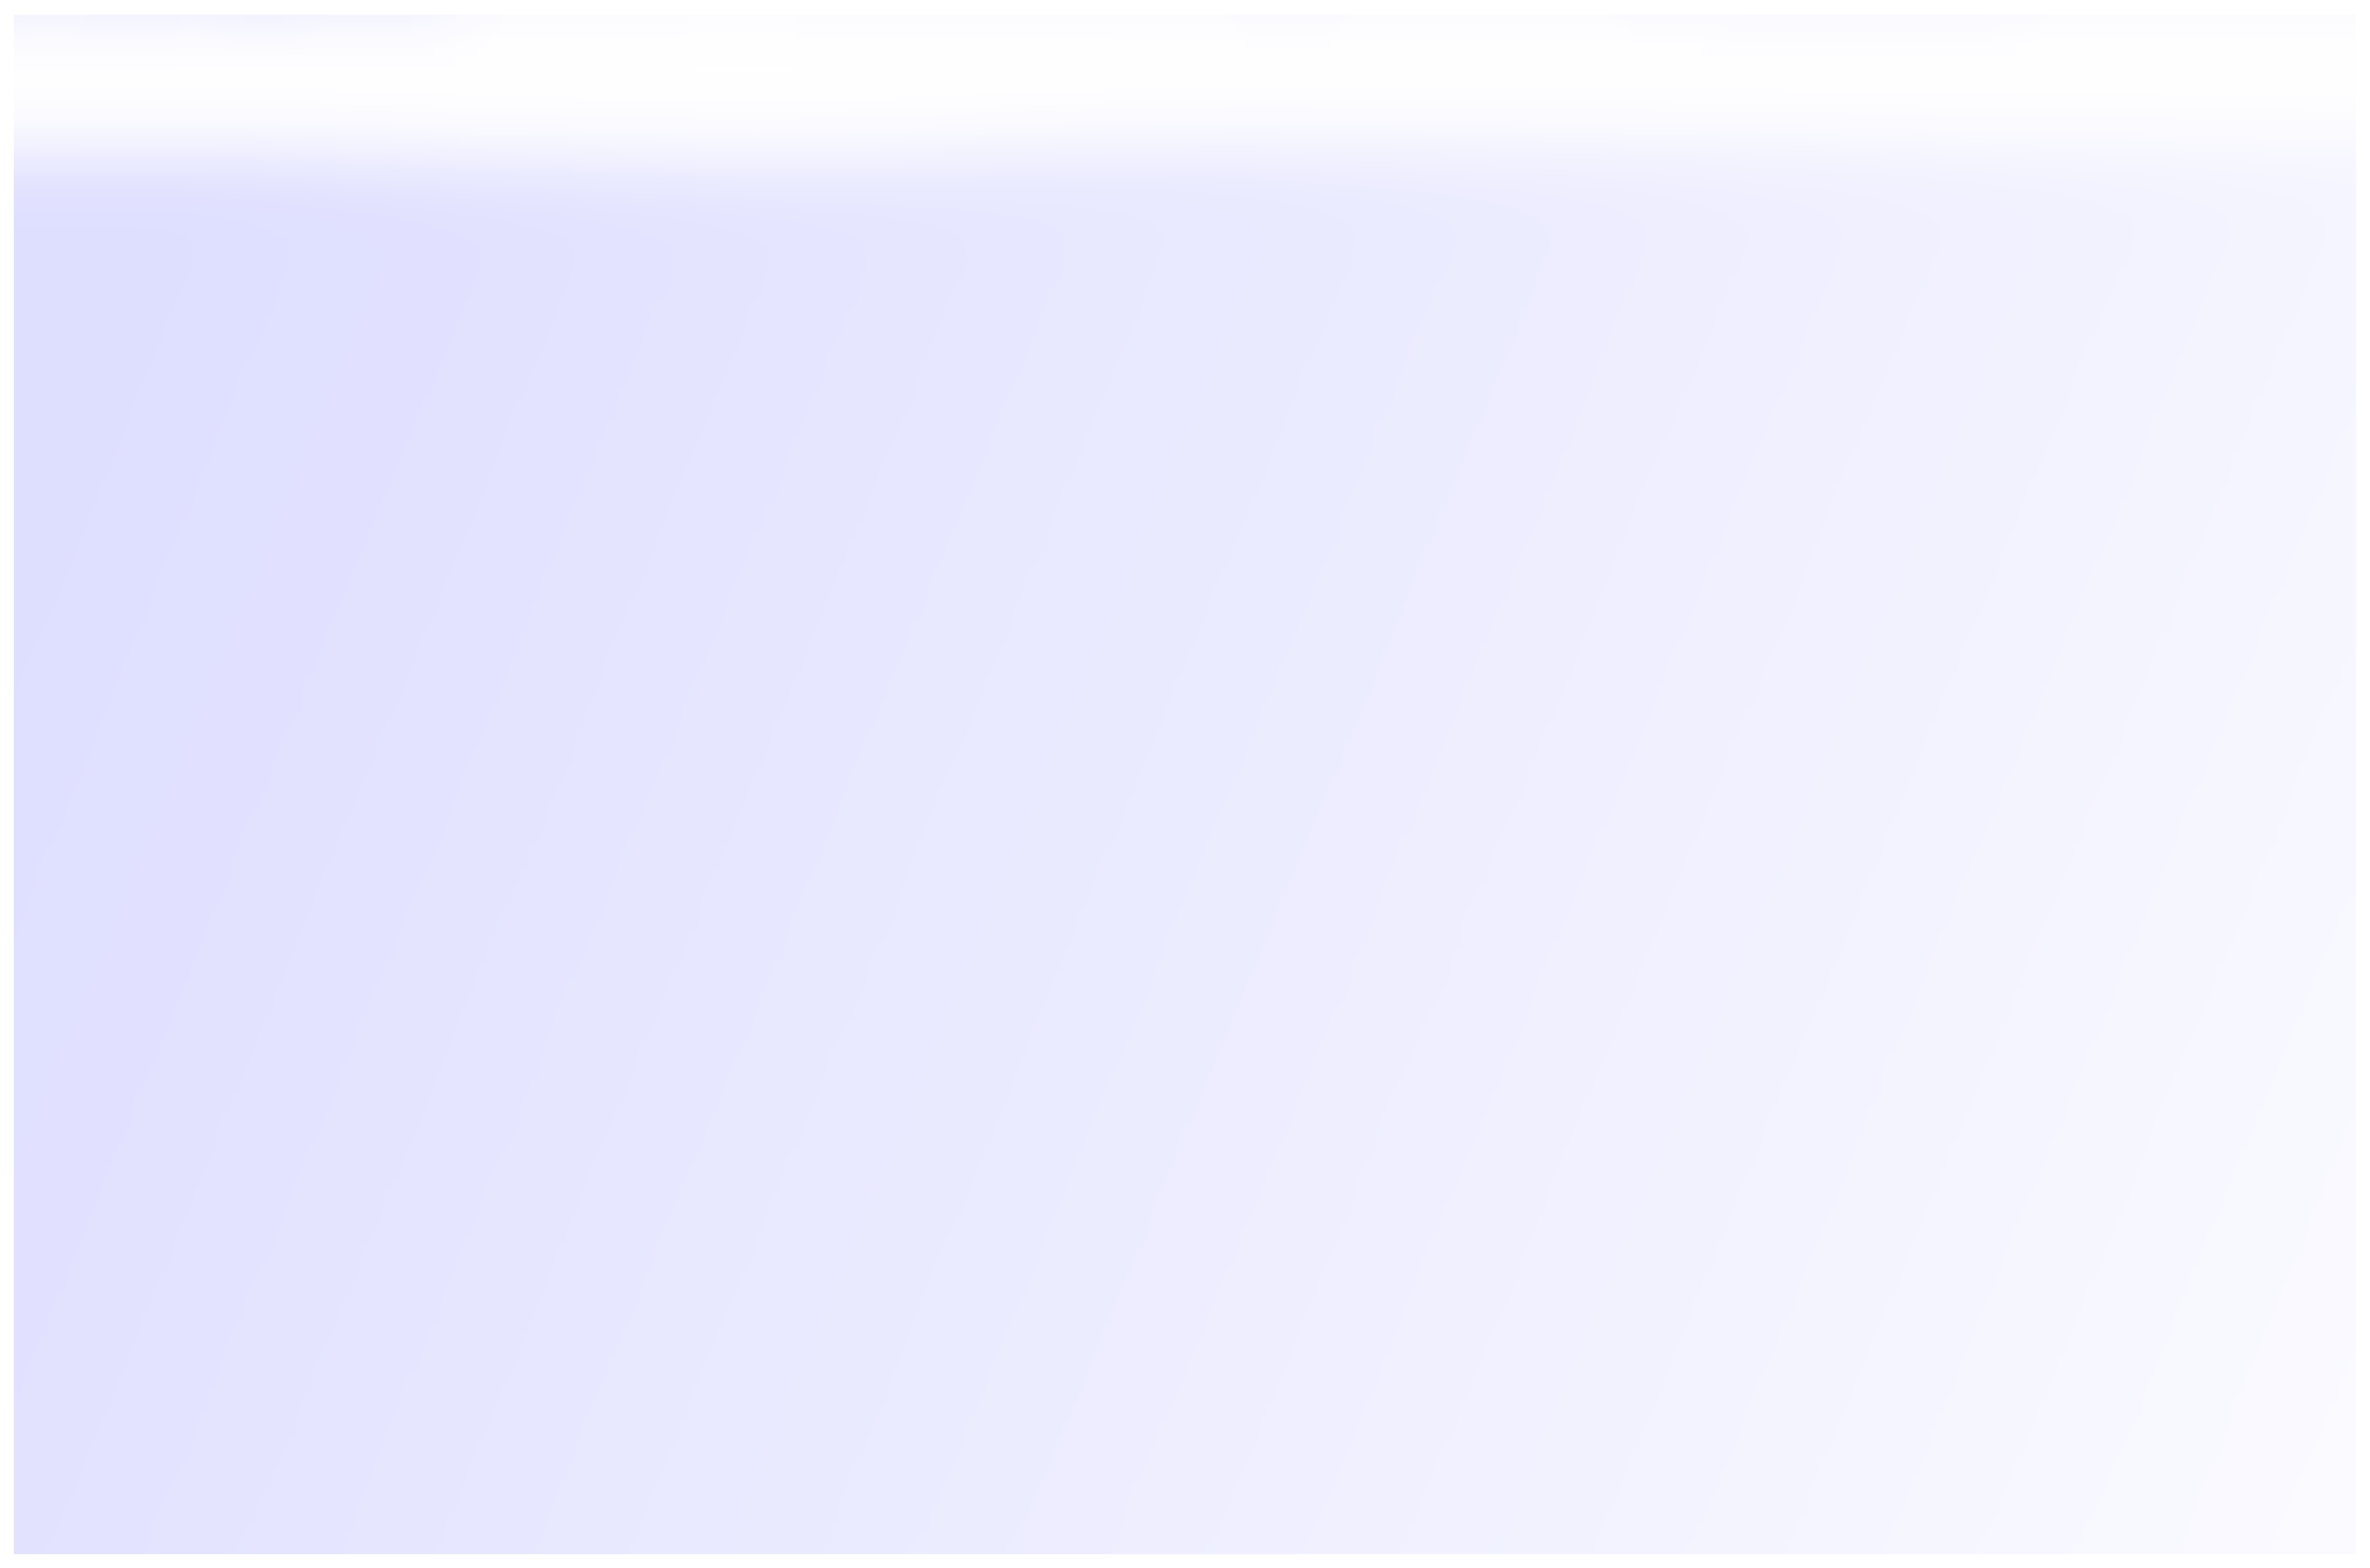
\includegraphics[height=1.1\textheight]{background}};
	\end{tikzpicture}
}

%%% General Poster Settings %%%%%%%%%%%%%%%%%%%%%%%%%%%%%%%%%%%%%%%%%%%%%%%%%%%
%%%%%% Eye Catcher, Title, Authors and University Images %%%%%%%%%%%%%%%%%%%%%%
\begin{poster}{
	grid=false,
	% Option is left on true though the eyecatcher is not used. The reason is
	% that we have a bit nicer looking title and author formatting in the headercol
	% this way
	%eyecatcher=false, 
	borderColor=bordercol,
	headerColorOne=headercol1,
	headerColorTwo=headercol2,
	headerFontColor=headerfontcol,
	% Only simple background color used, no shading, so boxColorTwo isn't necessary
	boxColorOne=boxcolor,
	headershape=roundedright,
	headerfont=\Large\sf\bf,
	textborder=rectangle,
	background=user,
	headerborder=open,
  boxshade=plain
}
%%% Eye Cacther %%%%%%%%%%%%%%%%%%%%%%%%%%%%%%%%%%%%%%%%%%%%%%%%%%%%%%%%%%%%%%%
{
	Eye Catcher, empty if option eyecatcher=false - unused
}
%%% Title %%%%%%%%%%%%%%%%%%%%%%%%%%%%%%%%%%%%%%%%%%%%%%%%%%%%%%%%%%%%%%%%%%%%%
{\sf\bf
    Simulation of a Software-Defined Network as One Big Switch
}
%%% Authors %%%%%%%%%%%%%%%%%%%%%%%%%%%%%%%%%%%%%%%%%%%%%%%%%%%%%%%%%%%%%%%%%%%
{
    \vspace{1em} Jiaqi Yan, Xin Liu, Dong (Kevin) Jin\\
    {\smaller \{jyan31, xliu125\}@hawk.iit.edu, dong.jin@iit.edu}
}
%%% Logo %%%%%%%%%%%%%%%%%%%%%%%%%%%%%%%%%%%%%%%%%%%%%%%%%%%%%%%%%%%%%%%%%%%%%%
{
% The logos are compressed a bit into a simple box to make them smaller on the result
% (Wasn't able to find any bigger of them.)
\setlength\fboxsep{0pt}
\setlength\fboxrule{0.5pt}
	\fbox{
		\begin{minipage}{15em}
			
\includegraphics[width=15em,height=4em]{iit_security_lab_logo}
		\end{minipage}
	}
}

\headerbox{Problem Statement}{name=problem,column=0,row=0}{
\begin{center}
    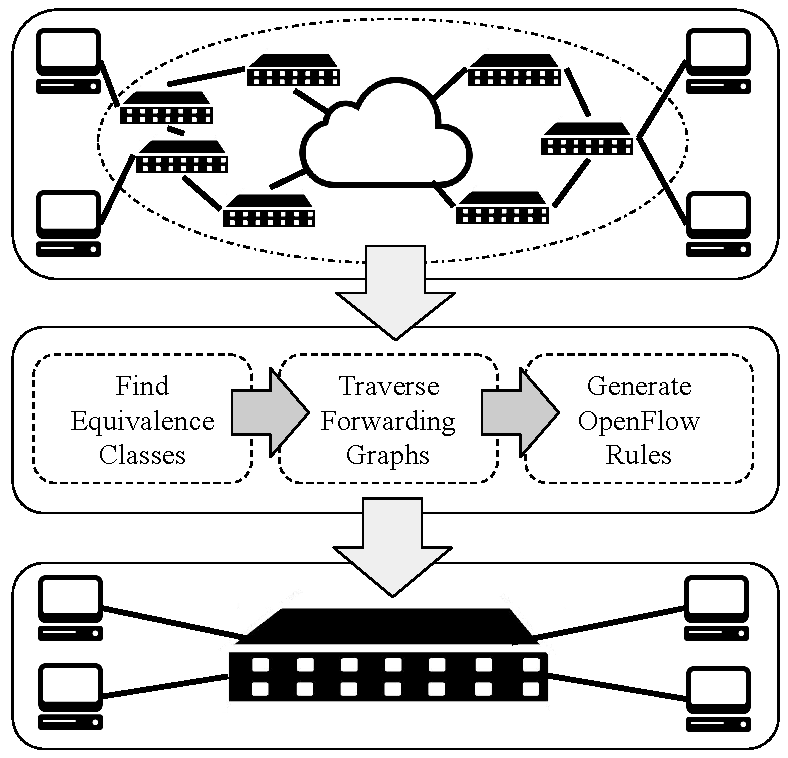
\includegraphics[width=\linewidth]{BigSimOverview}
\end{center}
Researchers have developed multiple SDN simulation and emulation platforms to expedite
the adoption of many emerging SDN-based applications to production systems.

However, the scalability of those platforms is often limited by the underlying physical
hardware resources, which inevitably affects the simulation fidelity in large-scale network settings.
In this work, we present a model abstraction technique that effectively transforms
the network devices in an SDN-based network to one virtualized switch model.
}

\headerbox{Application Scenarios}{name=motivation,column=0,below=problem}{
Our technique is useful if users only care about the end-to-end behavior rather than
the details within the network, applicable but not limited to the following scenarios:
    \begin{itemize}[leftmargin=1em]
        \item Simulate a large-scale \textbf{network of networks}.
        \item Deal with \textbf{synchronization} problem in hybrid simulation and emulation testbed
        \item Share SDN network models between collaborators as \textbf{plug-in}
    \end{itemize}
}

\headerbox{Approach Overhead}{name=overhead,column=0,below=motivation, above=bottom}{
\begin{center}
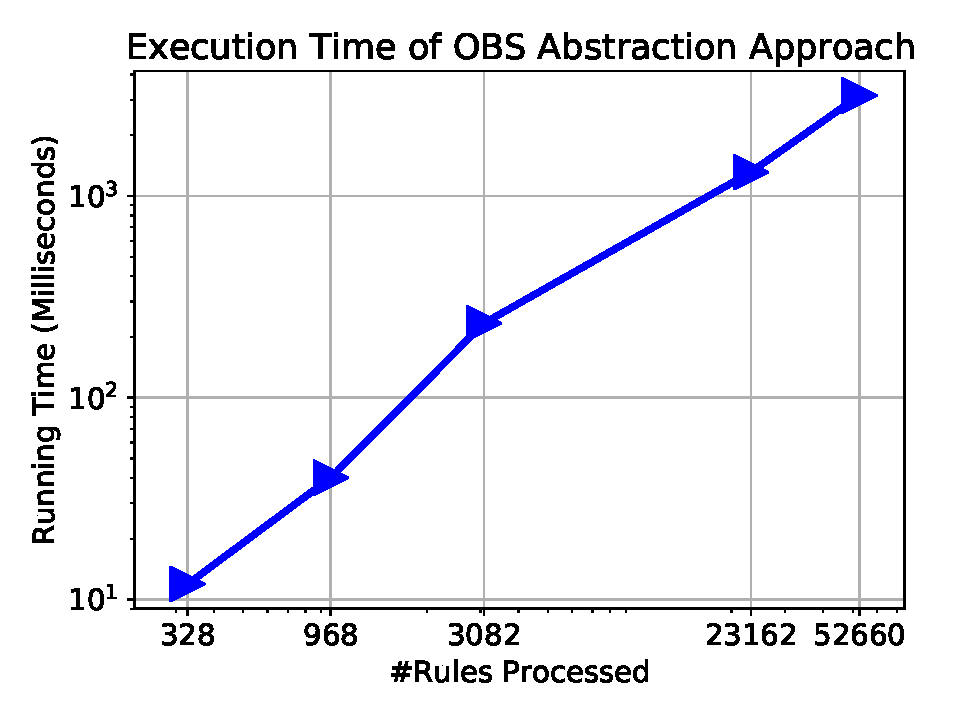
\includegraphics[angle=0,width=0.98\linewidth]{bs_overhead}
\end{center}
As the network state keeps evolving, it is essential to constantly update the abstracted
big-switch model to reflect the changes, preferably in an online fashion.
We recorded the running time for transforming various tree networks of different depth
and fanout into the one-big-switch network model.
The model abstraction process is lightweight.
For example, it took about 3.15 seconds to process 52,660 rules.
}

%\headerbox{References}{name=references,column=0,below=overhead, above=bottom}{
%\smaller													% Make the whole text smaller
%\vspace{-0.4em} 										% Save some space at the beginning
%\bibliographystyle{plain}							% Use plain style
%\renewcommand{\section}[2]{\vskip 0.05em}		% Omit "References" title
%\begin{thebibliography}{1}							% Simple bibliography with widest label of 1
%\itemsep=-0.01em										% Save space between the separation
%\setlength{\baselineskip}{0.4em}					% Save space with longer lines
%\bibitem{prevWork2} Laszlo Gulyas, Susan Khor, Richard Legendi and George Kampis \emph{Cumulative Properties of Elementary Dynamic Networks}, The International Sunbelt Social Network Conference XXXI (2011)
%\bibitem{gulya-kampis1} Gulyas, Laszlo et al.: \emph{Betweenness Centrality Dynamics in Networks of Changing Density}. Presented at the 19th International Symposium on Mathematical Theory of Networks and Systems (MTNS 2010)
%\end{thebibliography}
%}

\headerbox{Three-Step Model Abstraction Approach}{name=approach,span=2,column=1,row=0}{
To effectively transform a static SDN data plane configuration to ``one-big-switch" model
that preserves the same end-to-end forwarding behavior,
we need to identify how every packet is processed in the snapshot,
and how to correctly configure the big-switch model to reflect the identical forwarding logic.
We develop a three-step model abstraction method, summarized as follows.

    \begin{itemize}
    \item \textbf{Identifying Equivalence Classes (EC).}
        We partition all possible packets in the network into mutually exclusive sets
        and the packets belongs to the same EC are processed in the same way.
        Those sets are identified according to the matching field of \textbf{all}
        the OpenFlow rules on \textbf{all} the SDN switches in the original network.
    \item \textbf{Creating Forwarding Graphs.} We model the forwarding behavior of
        each packet set using the topology information as well as the local information
        stored on SDN switches (e.g., port mapping, rule priorities, etc),
        and generate a graph-based model to represent the forwarding behavior.
    \item \textbf{Generating OpenFlow Rules of the Big Switch.}
        We generate the OpenFlow rules for the big switch in order to preserve
        the end-to-end forwarding logic. This step includes (1) constructing the port-to-host mapping,
        (2) generating the rules by matching the packet header of each set,
        and (3) forwarding the packet to the correct output port.
    \end{itemize}

\begin{center}
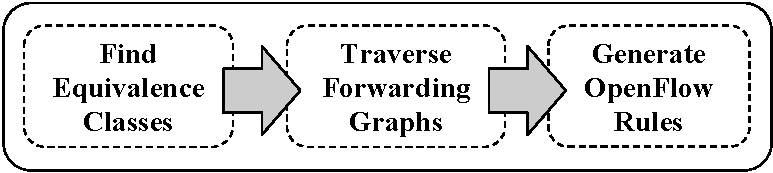
\includegraphics[angle=0,width=0.50\linewidth]{ThreeSteps}
\end{center}
}

\headerbox{Preserving Forwarding Logic}
{name=preserveForwardingLogic,span=2,column=1,below=approach}{
\begin{center}
	%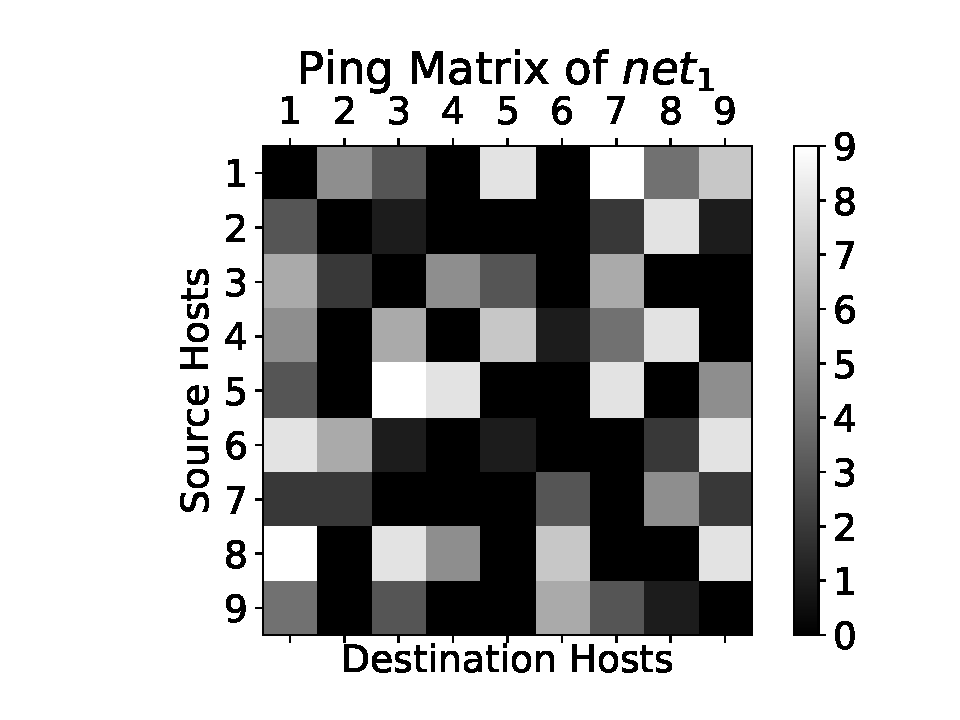
\includegraphics[angle=0,width=0.48\linewidth]{ping_mat_2_3}
	%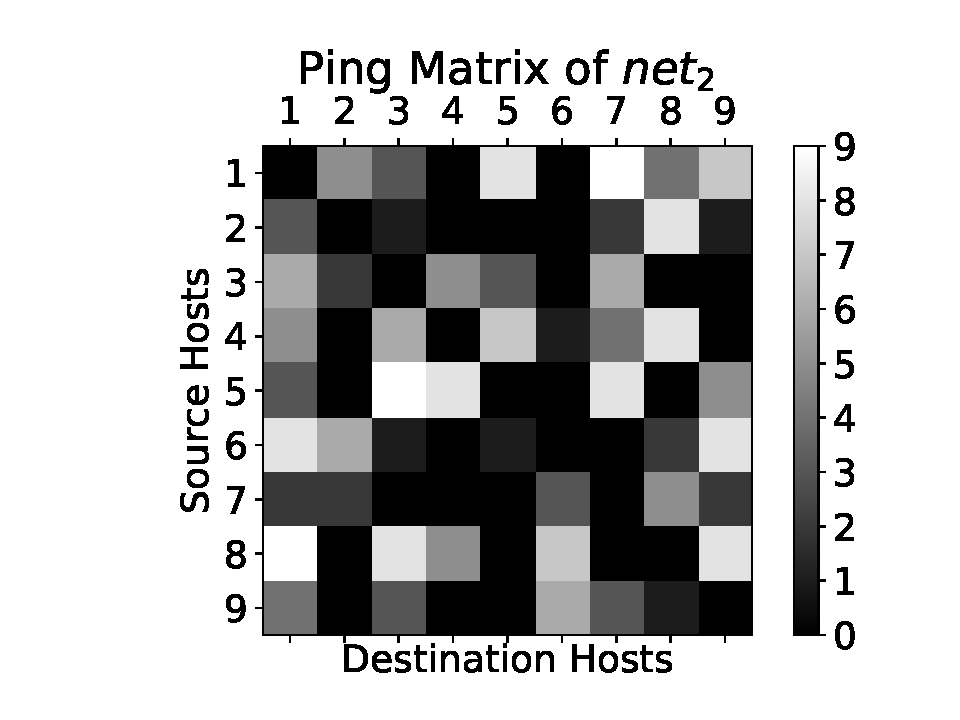
\includegraphics[angle=0,width=0.48\linewidth]{bs_ping_mat_2_3}
    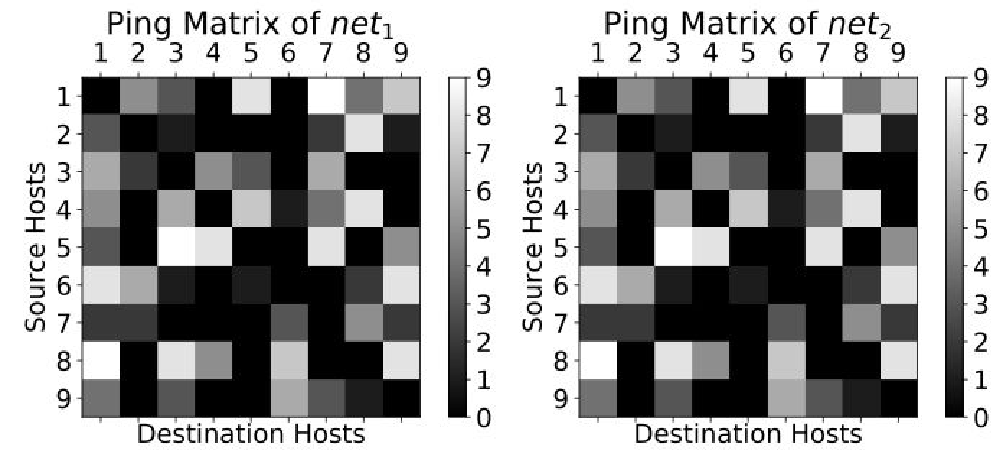
\includegraphics[angle=0,width=0.88\linewidth]{comp_ping_matrix}
\end{center}

$\mathbf{net_1}$ emulates the original SDN-based network with a tree topology ($d$, $f$),
where depth $d$ and fanout $f$ are tunable.
$\mathbf{net_2}$ emulates the corresponding one-big-switch-based network for each $net_1$
We conduct ping test between all combination of host-ends.
Matrix $\mathcal{R}_1$ and $\mathcal{R}_2$ represent the number of packets received at each host
in $net_1$ and $net_2$, respectively.
The gradient legend visualizes the number of received packets.
Identical $\mathcal{R}_1$ and $\mathcal{R}_2$ indicate that our model abstraction technique
preserves the network forwarding logic.
}

\headerbox{Performance Gain}
{name=performanceGain, span=2, column=1, below=preserveForwardingLogic, above=bottom}{

\begin{center}
	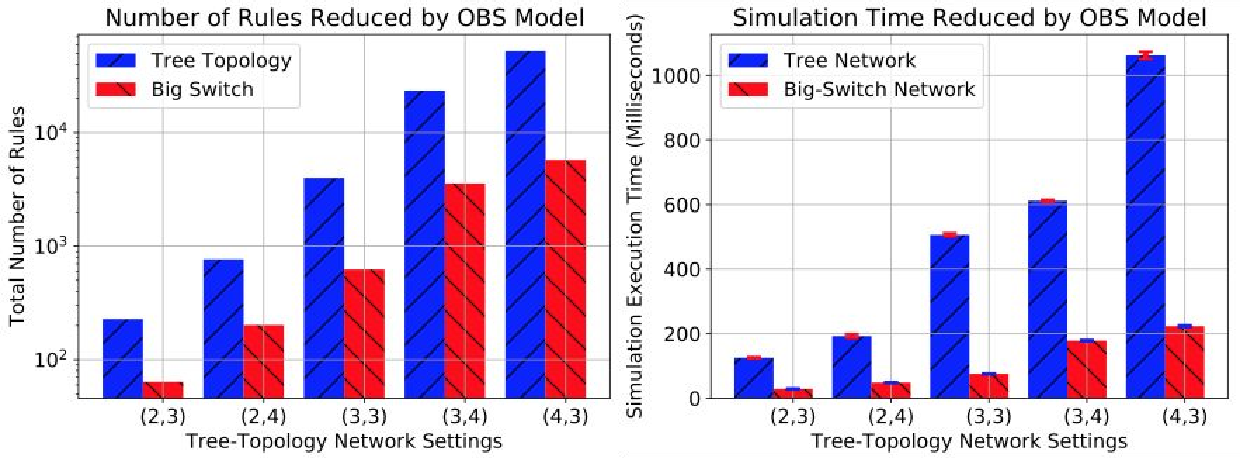
\includegraphics[angle=0,width=0.88\linewidth]{comp_both_rule_time}
	%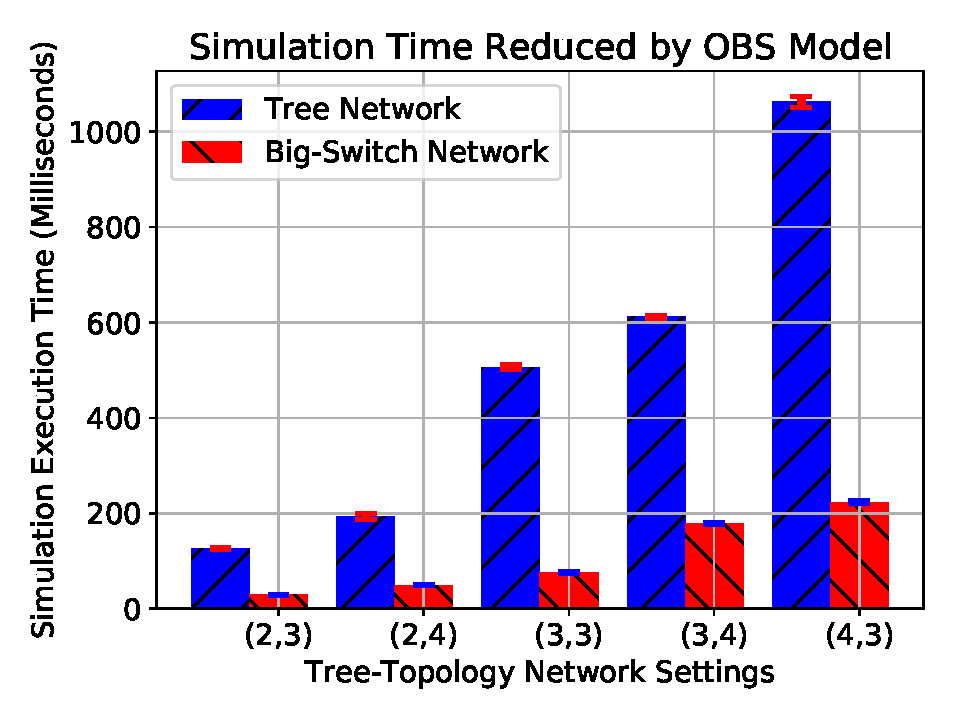
\includegraphics[angle=0,width=0.48\linewidth]{comp_sim_time}
\end{center}

\textbf{Number of OpenFlow Rules.} We compare the total number of rules installed
on the switches in both $net_1$ and $net_2$ with the same experimental settings.
The number of rules on the big switch is about 72\% to 89\% less than
the number of rules in the original tree-topology network.

\textbf{Simulation Running Time.}
When executing both models in the SDN simulator S3FNet,
the big-switch-based network model saves about 75\% to 85\% running time
as compared to simulating the corresponding original SDN-based network.

}
\end{poster}
\end{document}
